\documentclass{article}

\usepackage[paperwidth=8.5in,paperheight=11in,left=1.4in,
right=1in,top=1.3in, bottom=1.4in]{geometry}
\usepackage{sectsty, tikz, color, pgfplots}
\usetikzlibrary{shapes,arrows}
\usetikzlibrary{fit}
\makeatletter
\tikzset{
  fn/.style={
    inner sep=0pt,
    fill=none,
    draw=none,
    reset transform,
    fit={(\pgf@pathminx,\pgf@pathminy) (\pgf@pathmaxx,\pgf@pathmaxy)},
  },
  reset transform/.code={\pgftransformreset}
}
\makeatother

    \usetikzlibrary{patterns}
    \tikzset{%
        dotsfill/.style={draw,pattern=dots},
    }

\pgfdeclarepatternformonly[\StripesSize]{MyStripes}{\pgfqpoint{-1pt}{-1pt}}{\pgfqpoint{4pt}{4pt}}{\pgfqpoint{\StripesSize}{\StripesSize}}%
{
  \pgfsetlinewidth{0.3pt}
  \pgfpathmoveto{\pgfqpoint{0pt}{0pt}}
  \pgfpathlineto{\pgfqpoint{3.1pt}{3.1pt}}
  \pgfusepath{stroke}
}

\newdimen\StripesSize
\tikzset{
    StripesSize/.code={\StripesSize=#1},
    StripesSize=3pt
}

\begin{document}
\pagestyle{empty}
\begin{figure}
  \centering
    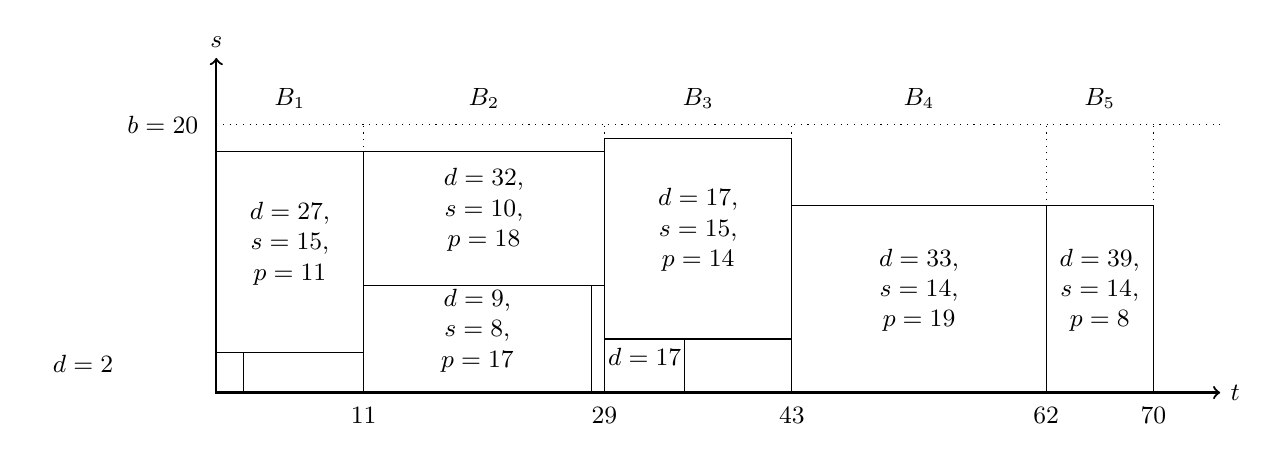
\begin{tikzpicture}[scale=0.17, font=\small]
      \draw [<->,thick] (0,25) node (yaxis) [above] {$s$}
        |- (75,0) node (xaxis) [right] {$t$};
      \draw[dotted] (0,20) -- (75,20);
      \node at (-4, 20) {$b = 20$};
        \draw (0,0) rectangle (2,3) node[fn, xshift=-5.3em, text width=4em] {$d = 2$};
        \draw (0,3) rectangle (11, 18) node[fn] {$d = 27,$\\ $s=15,$\\ $p = 11$};
        \node at (5.5, 22) {$B_1$};
        \node at (11, -1.7) {11};
      \draw[dotted] (11,0) -- (11,20); 
        \draw (11,0) rectangle (28, 8) node[fn] {$d = 9,$\\ $s=8,$\\ $p=17$};
        \draw (11,8) rectangle (29,18) node[fn] {$d = 32,$\\ $s=10,$\\ $p=18$};
        \node at (20, 22) {$B_2$};
        \node at (29, -1.7) {29};
      \draw[dotted] (29,0) -- (29, 20);
        \draw (29,0) rectangle (35,4) node[fn] {$d = 17$};
        \draw (29,4) rectangle (43,19) node[fn] {$d = 17,$\\ $s=15,$\\ $p=14$};
        \node at (36, 22) {$B_3$};
        \node at (43, -1.7) {43};
      \draw[dotted] (43,0) -- (43, 20);

        \draw (43,0) rectangle (62, 14) node[fn] {$d = 33,$\\ $s=14,$\\ $p=19$};
         \node at (52.5, 22) {$B_4$};
        \node at (62, -1.7) {62};

      \draw[dotted] (62,0) -- (62, 20);
        \draw (62,0) rectangle (70, 14) node[fn] (lastblock) {$d = 39,$\\
        $s=14,$\\ $p=8$};
         \node at (66, 22) {$B_5$};
        \node at (70, -1.7) {70};
      \draw[dotted] (70,0) -- (70, 20);

    \end{tikzpicture}
\end{figure}
\end{document}
